\documentclass[a4paper,14pt]{extarticle}
\usepackage{fontspec}
\usepackage{polyglossia}
\setmainlanguage{russian}
\setmainfont{Times New Roman}
\setmonofont{Courier New}[Scale=0.9]
\newfontfamily\cyrillicfont{Times New Roman}
\newfontfamily\cyrillicfonttt{Times New Roman}
\usepackage{geometry}
\geometry{left=2.5cm,right=1.5cm,top=2cm,bottom=2cm}
\usepackage{setspace}
\onehalfspacing
\usepackage{graphicx}
\usepackage{float}
\usepackage{caption}
\usepackage{enumitem}
\usepackage{booktabs}
\usepackage{longtable}
\usepackage{array}
\usepackage{hyperref}
\usepackage{xcolor}
\usepackage{listings}
\lstdefinestyle{cs}{
 language=[Sharp]C,
 basicstyle=\ttfamily\scriptsize,
 keywordstyle=\bfseries,
 commentstyle=\itshape,
 stringstyle=\itshape,
 numbers=left,
 numberstyle=\tiny,
 numbersep=6pt,
 frame=single,
 breaklines=true,
 showstringspaces=false,
 tabsize=4,
 columns=fullflexible,
 keepspaces=true,
 xleftmargin=2.2em,
 framexleftmargin=1.6em,
 aboveskip=8pt,
 belowskip=8pt
}
\lstdefinestyle{cmd}{
 basicstyle=\ttfamily\scriptsize,
 frame=single,
 breaklines=true,
 columns=fullflexible,
 keepspaces=true,
 showstringspaces=false,
 aboveskip=6pt,
 belowskip=6pt
}
\setlist{nosep,leftmargin=1.5em}
\captionsetup{font=small,skip=6pt}
\hypersetup{colorlinks=true,linkcolor=black,urlcolor=blue,pdftitle={Лабораторная работа 3. Цепной список}}
\begin{document}
\begin{titlepage}
\centering
\vspace*{2.2cm}
{\Large Лабораторная работа №\,3}\\[10pt]
по дисциплине\\
«Технологии промышленной разработки программного обеспечения.\\
Основные понятия»\\[18pt]
{\large Визуальный интерфейс к коллекции объектов\\
на односвязном списке}\\[56pt]
\begin{flushleft}
\hspace{0.42\textwidth}
\begin{tabular}{ll}
Выполнил: & студент группы М26-504\\[8pt]
& Гришанов Николай Вадимович\\
\end{tabular}
\end{flushleft}
\vfill
Москва — 2026
\end{titlepage}
\tableofcontents
\newpage
\section{Описание работы}
\subsection{Цель и постановка}
Цель работы — сделать оконное приложение, в котором коллекция объектов живёт в оперативной памяти и видна на форме. Объекты заданного типа хранятся в односвязном списке. Оператор создаёт список, добавляет элементы и перебирает их. Перебор должен идти через стандартные интерфейсы \texttt{IEnumerable<T>}, \texttt{IEnumerator<T>}, \texttt{IEnumerable} и \texttt{IEnumerator}, а не через отдельный обход полей формы.
По методическим указаниям тип элемента — \texttt{CheckBox} с видом кнопки. Кнопки стоят на панели с прокруткой. Смещение кнопки от левого края равно \texttt{40}, умноженному на номер, который возвращает \texttt{Append}. В строке состояния показываются короткие сообщения о результате команды.
\subsection{Что задано образцом и чего в нём нет}
Образец задаёт класс \texttt{MiniList<T>} с вставкой узла в голову и четыре команды меню: «Создать список», «Добавить элемент», «Перебор кнопок», «Перебор объектов». Обработчики написаны только для первых двух команд. Класс ещё не реализует перечислитель, поэтому \texttt{foreach} по списку невозможен.
Счётчик номеров объявлен как \texttt{static int num}. Он общий для всех списков одного закрытого типа и в образце не обнуляется. Поле \texttt{AutoSize} у \texttt{CheckBox} по умолчанию истинно, поэтому присваивание \texttt{Width = 30} без отключения авторазмера не удерживает узкую кнопку из образца.
\subsection{Принятое решение}
\texttt{MiniList<T>} реализует \texttt{IEnumerable<T>}. Вложенный перечислитель вручную хранит текущий узел и выполняет \texttt{MoveNext}, \texttt{Reset}, \texttt{Current} и \texttt{Dispose}. Отдельного итератора через \texttt{yield} нет: в задании требуется проверить все методы обоих интерфейсов.
Команда «Перебор кнопок» берёт перечислитель у необобщённого \texttt{IEnumerable}. Команда «Перебор объектов» берёт \texttt{IEnumerator<CheckBox>}. Оба проходят один и тот же список. Разница видна в строке состояния: «Кнопка: \ldots» или «Объект: \ldots». Текущая кнопка отмечается, панель прокручивается к ней. По завершении состояние отметок, которое было до команды, возвращается, а в строке состояния остаётся «O.K.».
Новый список заменяет старый: кнопки предыдущего списка снимаются с панели, потому что в новом списке их уже нет. Номер \texttt{num} при этом не сбрасывается, как в образце. Первая кнопка нового списка получает следующее смещение, а не ноль.
\section{Код}
Решение — два проекта SDK-стиля на .NET 10:
\begin{itemize}
\item \texttt{Lab3} — окно Windows Forms и класс \texttt{MiniList<T>};
\item \texttt{Lab3.Tests} — консольная проверка перечислителя, пишет протокол.
\end{itemize}
Файл решения: \texttt{Lab3.sln}.
\subsection{Точка входа}
\lstinputlisting[style=cs]{../Lab3/Program.cs}
\subsection{Список, перечислитель и форма}
\lstinputlisting[style=cs]{../Lab3/Form1.cs}
\subsection{Разметка окна}
\lstinputlisting[style=cs]{../Lab3/Form1.Designer.cs}
\subsection{Проверка интерфейсов}
\lstinputlisting[style=cs]{../Lab3.Tests/Program.cs}
\section{Описание написанного кода}
\subsection{MiniList<T>}
Класс повторяет образец. Узел \texttt{Node} хранит значение \texttt{content} и ссылку \texttt{Next}. Поле \texttt{Top} — голова списка. \texttt{Append} создаёт узел, ставит его перед прежней головой и возвращает \texttt{num++}. Из-за вставки в голову порядок перебора обратен порядку добавления: последняя кнопка на панели оказывается первой в списке.
\texttt{GetEnumerator} каждый раз создаёт новый перечислитель. Необобщённый метод интерфейса \texttt{IEnumerable} вызывает тот же обобщённый метод, поэтому оба меню обходят одни и те же узлы.
\subsection{Перечислитель}
Перечислитель помнит список, текущий узел и флаг \texttt{started}. До первого \texttt{MoveNext} флаг ложен, и чтение \texttt{Current} выбрасывает \texttt{InvalidOperationException}. Первый \texttt{MoveNext} берёт \texttt{Top}. Следующие переходят по \texttt{Next}. Когда узел кончился, \texttt{MoveNext} возвращает \texttt{false}, а \texttt{Current} снова запрещён. Повторный вызов за концом списка остаётся ложным. \texttt{Reset} возвращает перечислитель в положение «до первого элемента». \texttt{Dispose} ничего не освобождает: узлы принадлежат списку, а не обходу. Два перечислителя одного списка не мешают друг другу.
Необобщённое свойство \texttt{Current} возвращает тот же объект, что и обобщённое.
\subsection{Form1}
На форме — строка меню из четырёх команд, панель \texttt{panel1} с \texttt{AutoScroll = true} и строка состояния с пустой меткой. Это имена и свойства из указаний.
«Создать список» останавливает идущий перебор, очищает панель и записывает в поле \texttt{v} новый \texttt{MiniList<CheckBox>}. В строке состояния — «Список создан.» Очистка панели нужна потому, что старые кнопки к новому списку уже не относятся. Счётчик \texttt{num} команда не трогает.
«Добавить элемент» при пустой ссылке \texttt{v} пишет «Список не создан.» Иначе создаёт \texttt{CheckBox} с \texttt{Appearance.Button} и \texttt{FlatStyle.Standard}, отключает \texttt{AutoSize}, задаёт квадрат 30 на 30 и выравнивает подпись по центру. Левый край равен \texttt{40 * Append}. Подпись — это значение \texttt{Left}, как в образце. Узкая кнопка не вмещает три цифры целиком, поэтому на кнопке видна только часть числа. Полное значение показывает строка состояния во время перебора.
«Перебор кнопок» и «Перебор объектов» не стартуют, если списка нет или в нём нет узлов: сообщения «Список не создан.» и «Список пуст.» Перед проходом запоминаются отметки кнопок. Таймер с периодом 300~мс (80~мс, если кнопок больше 24) вызывает один шаг: \texttt{MoveNext}, отметка только у текущей кнопки, текст «Кнопка:» или «Объект:», прокрутка панели к этой кнопке. На последнем неудачном \texttt{MoveNext} перечислитель освобождается, отметки возвращаются, в строке состояния — «O.K.»
\section{Описание тестовых сценариев}
Проверяются два слоя.
Перечислитель проверяется без окна. Программа \texttt{Lab3.Tests} создаёт \texttt{MiniList<T>} и вызывает те же методы, что форма вызывает из меню: \texttt{Append}, \texttt{GetEnumerator}, \texttt{MoveNext}, \texttt{Current}, \texttt{Reset}, \texttt{Dispose}, а также \texttt{foreach} по обобщённому и необобщённому интерфейсу. Команда из каталога лабораторной:
\begin{lstlisting}[style=cmd]
dotnet run --project Lab3.Tests
\end{lstlisting}
Результат прогона: не пройдено 0, пройдено 19. Текст плана, результатов и заключения записан в \texttt{Протокол\_тестирования.txt}.
Окно проверяется отдельным прогоном по командам меню. После каждого контрольного состояния сохраняется снимок всего окна. Снимки лежат в \texttt{report/images} и приведены ниже. Снимок фиксирует меню, панель, отметку текущей кнопки, положение прокрутки и строку состояния.
Повторная съёмка:
\begin{lstlisting}[style=cmd]
dotnet run --project report/_capture -- report/images
\end{lstlisting}
Группы сценариев:
\begin{enumerate}
\item отказ добавления и перебора, пока список не создан;
\item пустой список: команда перебора не падает и сообщает, что список пуст;
\item ряд кнопок: смещение \texttt{40 * номер}, горизонтальная прокрутка, ручные отметки;
\item перебор кнопок с головы списка, то есть с последней добавленной кнопки, затем шаг к более ранним;
\item завершение прохода: «O.K.» и возврат прежних отметок;
\item перебор объектов тем же порядком, но с подписью «Объект:»;
\item новый список снимает старые кнопки и продолжает нумерацию;
\item контракт перечислителя на пустом списке, на списке из нескольких узлов, после \texttt{Reset} и при двух одновременных обходах.
\end{enumerate}
\section{Тестовые сценарии}
Ниже — сценарии, выполненные в окне. Ожидаемый текст строки состояния совпал с фактическим.
\subsection{Старт}
Шаги: запустить приложение.\\
Ожидание: меню из четырёх команд, панель пустая, строка состояния пустая.\\
Факт: совпало, рисунок~\ref{fig:start}.
\begin{figure}[H]
\centering
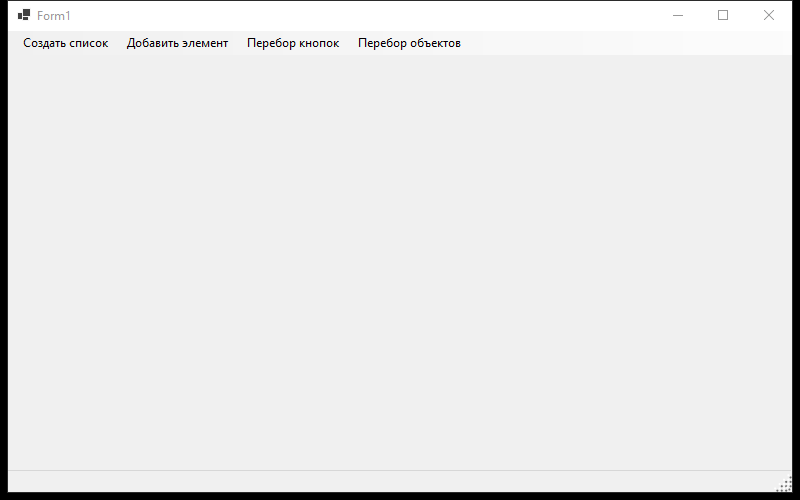
\includegraphics[width=\textwidth]{images/01-start.png}
\caption{Окно сразу после запуска}
\label{fig:start}
\end{figure}
\subsection{Добавление без списка}
Шаги: не создавая список, выбрать «Добавить элемент».\\
Ожидание: панель пустая, в строке состояния «Список не создан.»\\
Факт: совпало, рисунок~\ref{fig:nolist}.
\begin{figure}[H]
\centering
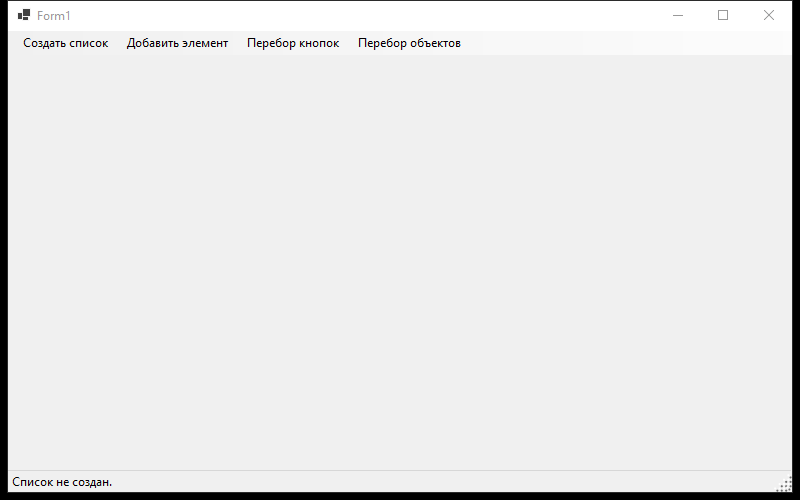
\includegraphics[width=\textwidth]{images/02-no-list.png}
\caption{Отказ добавить кнопку до создания списка}
\label{fig:nolist}
\end{figure}
\subsection{Создание списка}
Шаги: выбрать «Создать список».\\
Ожидание: панель по-прежнему пустая, в строке состояния «Список создан.»\\
Факт: совпало, рисунок~\ref{fig:created}.
\begin{figure}[H]
\centering
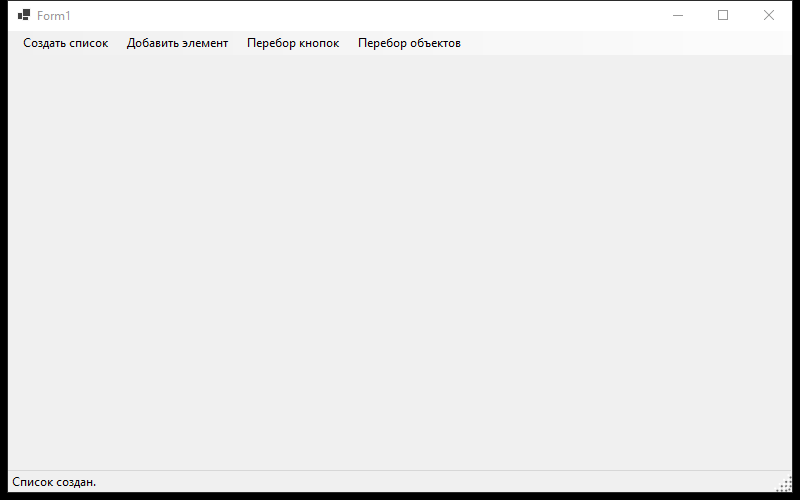
\includegraphics[width=\textwidth]{images/03-created.png}
\caption{Список создан, узлов ещё нет}
\label{fig:created}
\end{figure}
\subsection{Перебор пустого списка}
Шаги: при только что созданном списке выбрать «Перебор кнопок».\\
Ожидание: «Список пуст.», исключение не возникает.\\
Факт: совпало, рисунок~\ref{fig:empty}.
\begin{figure}[H]
\centering
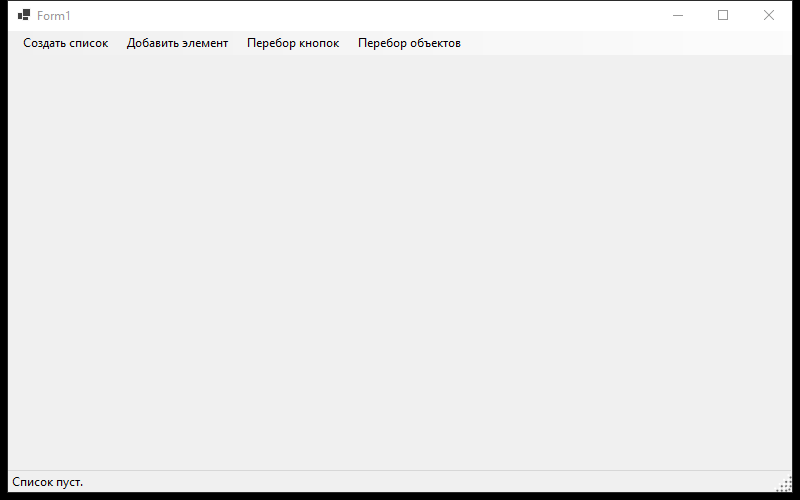
\includegraphics[width=\textwidth]{images/04-empty.png}
\caption{Перебор не начат: в списке нет узлов}
\label{fig:empty}
\end{figure}
\subsection{Ряд кнопок}
Шаги: двадцать два раза выбрать «Добавить элемент». Отметить кнопки со смещением 80 и со смещениями от 160 до 400 включительно.\\
Ожидание: подписи равны смещению \texttt{0, 40, 80, \ldots, 840}. Кнопки шириной 30 не показывают все цифры чисел от 100. Внизу панели — горизонтальная прокрутка. Отмечены кнопка 80 и кнопки 160--400. Строка состояния пустая: добавление её очищает.\\
Факт: совпало, рисунок~\ref{fig:buttons}. На видимом участке подпись 120 обрезана до «12», 160 — до «16», 400 — до «40».
\begin{figure}[H]
\centering
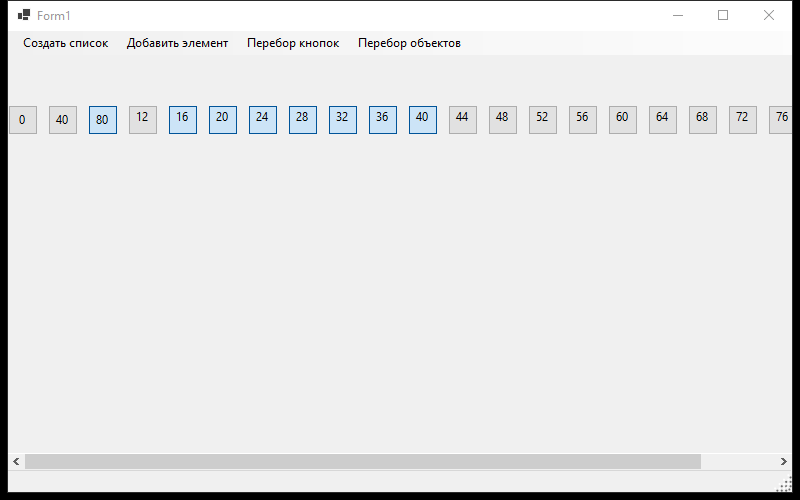
\includegraphics[width=\textwidth]{images/05-buttons.png}
\caption{Двадцать две кнопки, часть отмечена вручную}
\label{fig:buttons}
\end{figure}
\subsection{Перебор кнопок с головы списка}
Шаги: выбрать «Перебор кнопок» и остановить проход на первом узле.\\
Ожидание: голова списка — последняя добавленная кнопка, смещение 840. Панель прокручена вправо. Отмечена только она. Строка состояния — «Кнопка: 840».\\
Факт: совпало, рисунок~\ref{fig:walk}. На кнопке из-за ширины 30 виден фрагмент «84».
\begin{figure}[H]
\centering
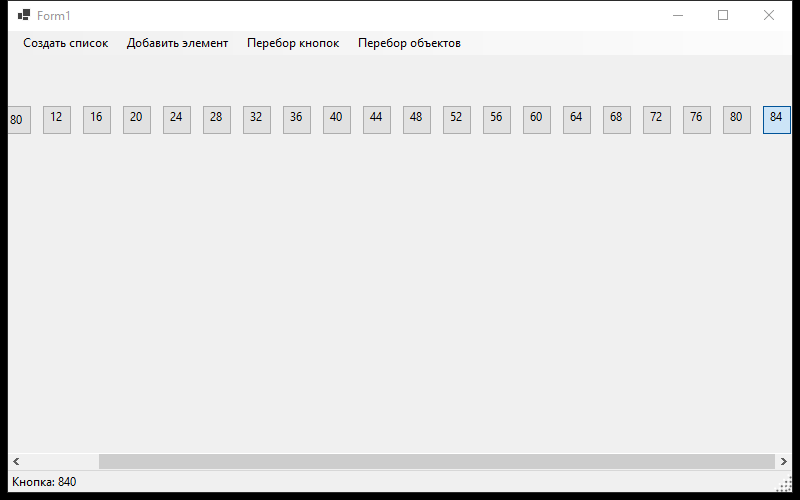
\includegraphics[width=\textwidth]{images/06-walk-button.png}
\caption{Первый шаг необобщённого перечислителя}
\label{fig:walk}
\end{figure}
Шаги: сделать ещё шесть шагов того же прохода.\\
Ожидание: текущее смещение \texttt{840 - 6 * 40 = 600}, строка «Кнопка: 600», отмечена одна кнопка.\\
Факт: совпало, рисунок~\ref{fig:middle}.
\begin{figure}[H]
\centering
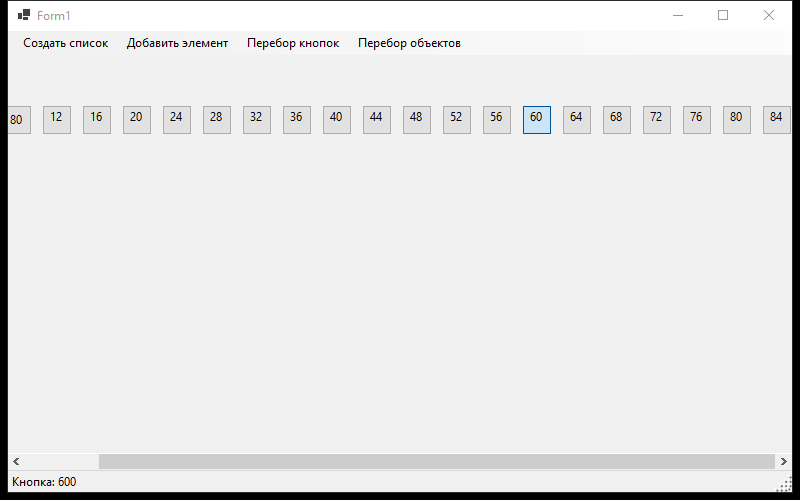
\includegraphics[width=\textwidth]{images/07-walk-middle.png}
\caption{Шестой шаг после головы: кнопка 600}
\label{fig:middle}
\end{figure}
\subsection{Завершение прохода}
Шаги: дойти до конца того же перебора.\\
Ожидание: строка состояния «O.K.», отметки вернулись к состоянию до команды (80 и 160--400), прокрутка снова показывает левый край.\\
Факт: совпало, рисунок~\ref{fig:ok}.
\begin{figure}[H]
\centering
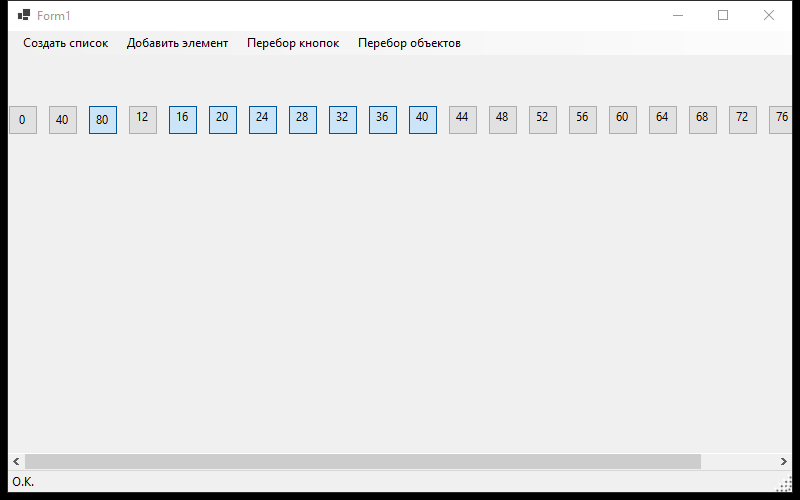
\includegraphics[width=\textwidth]{images/08-ok.png}
\caption{После прохода отметки восстановлены}
\label{fig:ok}
\end{figure}
\subsection{Перебор объектов}
Шаги: выбрать «Перебор объектов» и перейти на третий узел.\\
Ожидание: порядок тот же, что у кнопок. Первый узел — 840, третий — 760. Строка состояния — «Объект: 760», отмечена одна кнопка.\\
Факт: совпало, рисунок~\ref{fig:object}.
\begin{figure}[H]
\centering
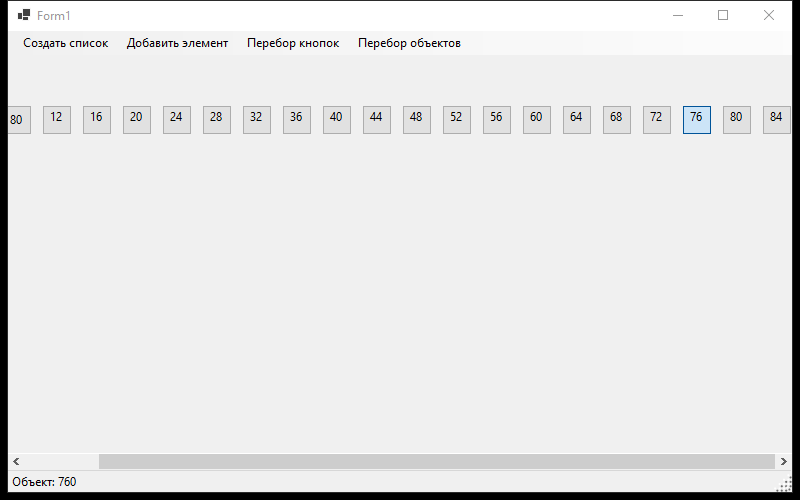
\includegraphics[width=\textwidth]{images/09-walk-object.png}
\caption{Обобщённый перечислитель, третий узел}
\label{fig:object}
\end{figure}
\subsection{Новый список продолжает нумерацию}
Шаги: завершить перебор, выбрать «Создать список», затем два раза «Добавить элемент» и прокрутить панель к новым кнопкам.\\
Ожидание: прежние двадцать две кнопки сняты. Счётчик после них равен 22, поэтому новые смещения — 880 и 920. Строка состояния пустая, потому что её очищает добавление.\\
Факт: совпало, рисунок~\ref{fig:newlist}. На кнопках видны обрезанные «88» и «92».
\begin{figure}[H]
\centering
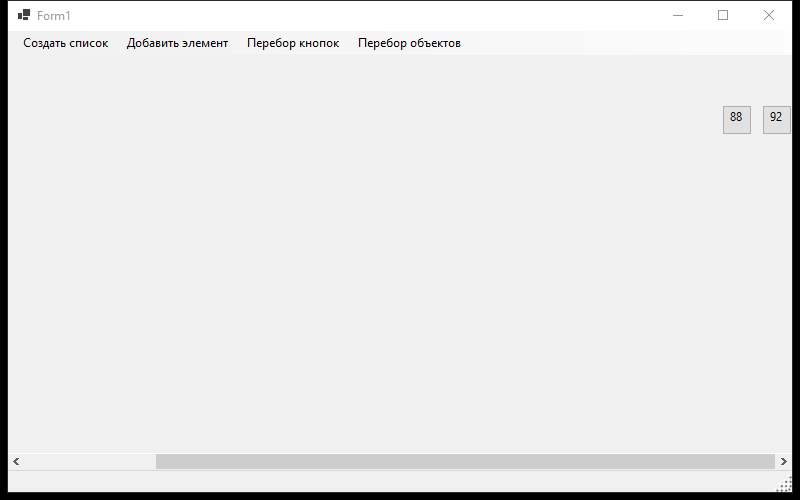
\includegraphics[width=\textwidth]{images/10-new-list.png}
\caption{Новый список: старые кнопки сняты, номера продолжаются}
\label{fig:newlist}
\end{figure}
\subsection{Сценарии, закрытые только проверкой перечислителя}
\begin{center}
\begin{tabular}{p{0.42\textwidth}p{0.24\textwidth}p{0.22\textwidth}}
\toprule
Проверка & Ожидание & Результат\\
\midrule
\texttt{Current} до \texttt{MoveNext} на пустом списке & исключение & пройден\\
\texttt{MoveNext} на пустом списке & \texttt{false} & пройден\\
\texttt{Current} после этого \texttt{MoveNext} & исключение & пройден\\
три вызова \texttt{Append} & номера \(n\), \(n+1\), \(n+2\) & пройден\\
голова и хвост после \texttt{a}, \texttt{b}, \texttt{c} & \texttt{c}, затем \texttt{b}, затем \texttt{a} & пройден\\
\texttt{foreach} по \texttt{MiniList<int>} & 3, 2, 1 & пройден\\
\texttt{foreach} по \texttt{IEnumerable} & та же последовательность & пройден\\
необобщённый \texttt{Current} & то же значение & пройден\\
\texttt{Reset} после полного прохода & повтор даёт прежний первый элемент & пройден\\
\texttt{MoveNext} за последним узлом дважды & оба раза \texttt{false} & пройден\\
два перечислителя одного списка & каждый хранит свой узел & пройден\\
\texttt{Dispose} & исключения нет & пройден\\
\bottomrule
\end{tabular}
\end{center}
\section{Документация}
\subsection{Руководство оператора}
Запуск: \texttt{dotnet run --project Lab3}. Открывается одно окно.
Сначала выбирают «Создать список». Пока этой команды не было, «Добавить элемент» и обе команды перебора только пишут причину отказа в строку состояния.
«Добавить элемент» ставит справа следующую кнопку. Если ряд уходит за край панели, внизу появляется горизонтальная прокрутка. Щелчок по кнопке отмечает её и снимает отметку: это обычное поведение \texttt{CheckBox} с видом кнопки и к списку не относится.
«Перебор кнопок» и «Перебор объектов» по очереди отмечают узлы списка, начиная с последней добавленной кнопки и двигаясь к первой. В строке состояния видно полное смещение, даже если на узкой кнопке число обрезано. Когда проход закончен, прежние отметки возвращаются и появляется «O.K.» Повторная команда начинает проход сначала. «Создать список» во время прохода прерывает его и убирает кнопки.
\subsection{Сборка}
Нужен SDK .NET 10 с поддержкой Windows Forms. Из каталога лабораторной:
\begin{lstlisting}[style=cmd]
dotnet run --project Lab3.Tests
dotnet run --project Lab3
\end{lstlisting}
Отчёт собирается XeLaTeX из каталога \texttt{report} (нужны \texttt{polyglossia}, \texttt{fontspec}, \texttt{listings}):
\begin{lstlisting}[style=cmd]
xelatex lab3_report.tex
xelatex lab3_report.tex
\end{lstlisting}
Второй проход нужен для оглавления.
\subsection{Ограничения}
Удалить один узел или сохранить список на диск нельзя: в задании этого нет. Подпись на кнопке обрезается, потому что ширина 30 взята из образца. Перебор идёт от последней кнопки к первой, потому что \texttt{Append} вставляет узел в голову. Новый список не начинает нумерацию с нуля: статический счётчик образца этого не делает, и сброс в программу не добавлялся. Во время прохода отметка кнопки занята подсветкой текущего узла; после «O.K.» возвращается то, что оператор отметил сам.
\subsection{Состав поставки}
\begin{center}
\begin{tabular}{p{0.46\textwidth}p{0.46\textwidth}}
\toprule
Путь & Назначение\\
\midrule
\texttt{Lab3.sln} & решение\\
\texttt{Lab3} & окно и \texttt{MiniList<T>}\\
\texttt{Lab3.Tests} & 19 проверок перечислителя\\
\texttt{Протокол\_тестирования.txt} & план, результаты и заключение прогона\\
\texttt{report/lab3\_report.tex} & настоящий отчёт\\
\texttt{report/images} & снимки сценариев\\
\texttt{report/\_capture} & повторная съёмка окна\\
\bottomrule
\end{tabular}
\end{center}
\section*{Заключение}
\addcontentsline{toc}{section}{Заключение}
По образцу лабораторной собрано окно с меню, прокручиваемой панелью кнопок и строкой состояния. Коллекция \texttt{CheckBox} хранится в односвязном списке \texttt{MiniList<T>} с вставкой в голову. Список отдаёт элементы через обобщённый и необобщённый перечислители. «Перебор кнопок» и «Перебор объектов» показывают один и тот же порядок узлов и различаются интерфейсом, через который этот порядок получен. По окончании прохода строка состояния содержит «O.K.», а отметки кнопок возвращаются. Контракт \texttt{MoveNext}, \texttt{Current}, \texttt{Reset} и \texttt{Dispose} закрыт 19 проверками. Поведение окна закрыто десятью снимками: отказ до создания списка, пустой список, ряд кнопок, оба вида перебора и новый список с продолжением нумерации.
\end{document}
